\chapter{Projekt systemu}

Opracowany system składa się z dwóch zasadniczych części: programu przeznaczonego dla komputera PC, służącego do tworzenia animacji oraz urządzenia elektronicznego, które te animacje wyświetla. Między tymi składowymi systemu wymieniane są dane w~postaci plików MXF i~M2F. W~dalszej części rozdziału przedstawiono ich format.

\section{Wymagania funkcjonalne i~pozafunkcjonalne}

Poniżej zamieszczono zbiór wymagań, jakie postawione zostały przed urządzeniem oraz programem do tworzenia animacji. Z~racji niskiego skomplikowania interfejsu użytkownika tablicy świetlnej ograniczono się do ogólnego ich sformułowania. Dla programu komputerowego podzielono je na funkcjonalne oraz pozafunkcjonalne.

\subsection{Wymagania dla tablicy świetlnej}

System:
\begin{itemize}
	\item umożliwia wyświetlanie animacji zgodnych z~formatami MXF i~M2F,
	\item odczytuje animacje z~karty SD,
	\item umożliwia manipulacje zawartością karty SD poprzez port USB,
	\item sterowany jest przy użyciu dwóch przycisków,
	\item zapewnia możliwość wyboru pliku z~animacją i~otwarcia go,
	\item umożliwia używanie tablicy bez karty pamięci,
	\item umożliwia ustawienie godziny i~daty,
	\item jest dostosowany do wydajności mikroprocesora.
\end{itemize}

\newpage 

\subsection{Wymagania dla aplikacji użytkownika}

System umożliwia użytkownikowi:
\begin{itemize}
	\item zaprojektowanie układu graficznego wyświetlanego na tablicy,
	\item zarządzanie elementami projektu --- usuwanie obszarów, zmiana ich typu, edycja zawartości,
	\item wyeksportowanie pliku końcowego, który zostanie prawidłowo zinterpretowany przez wykonany moduł i~w~pełni spójny z~projektem użytkownika,
	\item zapisywanie aktualnego projektu do pliku, otwieranie, edytowanie i~nadpisywanie istniejących projektów,
	\item wizualizację aktualnego projektu lub wygenerowanych wcześniej plików końcowych poprzez symulator.
\end{itemize}

Ponadto, realizując wymagania pozafunkcjonalne, system:
\begin{itemize}
	\item zapewnia nieskomplikowaną, intuicyjną i~szybką obsługę,
	\item informuje o~ograniczeniach związanych z~tworzeniem animacji. W~razie konieczności uniemożliwia wykonanie operacji.
\end{itemize}

\section{Pliki z~animacjami}
Ekran obsługuje dwa formaty plików: M2F i~MXF.~Podrozdziały \ref{m2f-desc} i~\ref{mxf-desc} są poświęcone opisowi tych plików. Oprócz nich zdefiniowano format MMF, który używany jest wyłącznie przez program komputerowy do do zapisu edytowalnego projektu i~nie jest przedmiotem niniejszego rozdziału.

\subsection{Pliki M2F}
\label{m2f-desc}
Dla pliku służącego do wymiany danych między urządzeniem i~komputerem określono następujące wymagania: 
\begin{enumerate}
	\item możliwość wypisania aktualnej daty i~czasu,
	\item możliwość wyświetlania grafiki,
	\item możliwość wyświetlania tekstu i~grafiki jednocześnie,
	\item dodatkowe możliwości, między innymi wyświetlanie w~pionie,
	\item różne czcionki,
	\item mały rozmiar plików,
	\item mała wymagana moc obliczeniowa przy odtwarzaniu,
	\item plik nie musi być czytelny dla człowieka.
\end{enumerate}
W ramach realizacji tych założeń powstał format M2F.~Nazwa ma sugerować, że opisuje on to samo, co plik MMF, tylko w~inny sposób. Cała metoda wyświetlania bazuje przede wszystkim na buforze tła i~opisie liter. Co pewien czas jest generowana nowa klatka. Na początku wczytywane są komendy sterujące, modyfikujące tło, opis liter. Potem tworzy się kopię tła i~nanosi na nią po kolei zdefiniowane litery. Litery mogą nachodzić na siebie nadpisując się. Gotowa klatka zostaje narysowana. W~kolejnych podpunktach znajdują się opisy poszczególnych elementów formatu oraz bardziej szczegółowy opis.

\subsection{Komendy}
\subsubsection*{Komendy sterujące}
Komendy sterujące jako pierwszy bajt mają wartość 0. Drug bajt jest numerem komendy. Obecnie są dostępne 22 komendy:
\begin{itemize}
\item 0 --- koniec pliku (plik po zakończeniu jest odczytywany jako ciąg zer, czyli nie musi zawierać tej komendy),
\item 1 --- koniec danych dla klatki, czyli odczekaj 1 klatkę,
\item 2 --- odczekaj 2 klatki,
\item 3 --- odczekaj 5 klatek,
\item 4 --- odczekaj 10 klatek,
\item 5 --- odczekaj 20 klatek,
\item 6 --- odczekaj 50 klatek,
\item 7 --- odczekaj 100 klatek,
\item 8 --- czekaj do końca sekundy,
\item 9 --- czekaj do końca minuty,
\item 10 --- czekaj do końca godziny,
\item 11 --- czekaj do końca dnia,
\item 12 --- nie rysuj nic,
\item 13 --- rysuj tylko litery (domyślnie animacja rozpoczyna się z~takim ustawieniem),
\item 14 --- rysuj tylko tło,
\item 15 --- rysuj litery i~tło,
\item 16 --- gdy tło nie jest rysowane, rysuj na pustej klatce (domyślnie animacja rozpoczyna się z~takim ustawieniem),
\item 17 --- gdy tło nie jest rysowane, rysuj na wypełnionej klatce,
\item 18 --- modyfikacja tła (składnia jest opisana poniżej),
\item 19 --- czekaj na przycisk,
\item 20 --- przewiń plik do początku (stan znaków, tła i~przełączników nie jest przywracany do stanu początkowego),
\item 21 --- przywrócenie ustawień początkowych wyświetlania, opisanych w~dziale \ref{algorithm-description}.
\end{itemize}

\subsubsection*{Składnia instrukcji modyfikującej tło}
Odczytywane są kolejne 2 bajty z~pliku, które opisują w~którym miejscu tło ma zostać modyfikowane. Modyfikuje się obraz w~podziale na obszary o~wymiarach i~położeniu będących wielokrotnościami liczby 16. Pierwszy bajt podaje współrzędne początkowe, drugi współrzędne końcowe. Cztery bardziej znaczące bity oznaczają położenie w~pionie, pozostałe położenie w~poziomie. Wartości z~tych bitów są mnożone przez 16. Odczytanie wartości 0x01 i~0x13 oznacza, że zmodyfikowany zostanie obszar o~współrzędnej X od 16 do 48 i~o~współrzędnej Y od 0 do 16. Obszar ten zawiera 512 pikseli, czyli jest opisany 512 bitami, czyli 64 bajtami. Każde 2 bajty stanowią szesnastobitową kolumnę obrazu, pierwszy bajt jest bardziej znaczący. Na ekranie piksele na dole odpowiadają bardziej znaczącym bitom. Dla przykładowych bajtów 0x33 i~0xf0 postanie kolumna (od dołu) 0011001111110000. Gdyby obszar był wyższy niż 16 pikseli, dane byłyby podane w~pasach, na przykład dla pierwszych dwóch bajtów 0x01 i~0x23, najpierw X od 16 do 48, Y od 0 do 16; potem X od 16 do 48, Y od 16 do 32.

\subsubsection*{Komendy modyfikujące litery}
Komendy tego rodzaju rozpoczynają się bajtem większym od zera, oznaczającym numer litery, po którym jest numer parametru i~jego nowa wartość. Można modyfikować następujące parametry:
\begin{itemize}
\item 0 --- kod znaku (opis użytego kodowania znajduje się poniżej),
\item 1 --- położenie w~poziomie (może być ujemne, liczone od lewej strony),
\item 2 --- położenie w~pionie (może być ujemne, liczone od góry),
\item 3 --- tryb wyświetlania (opis trybów znajduje się poniżej),
\item 4 --- czcionka (opis czcionek znajduje się poniżej)
\item 5 --- przycięcie znaku w~poziomie, od ile,
\item 6 --- przycięcie znaku w~pionie, od ile,
\item 7 --- przycięcie znaku w~poziomie, do ile,
\item 8 --- przycięcie znaku w~pionie, do ile (opis przycięć znajduje się poniżej).
\end{itemize}

\subsection{Kodowanie znaków}
Użyte kodowanie jest częściowo zgodne z~ASCII.~Są kompatybilne od znaku 32 (spacja) do 126 (tylda). Z~założenia to kodowanie zawiera wszystkie znaki powszechnie używane w~języku polskim. Zawiera również aktywne znaki służące do opisu aktualnej daty i~czasu. Oprócz kodowania zgodnego z~ASCII, w~ramach pozostałych kodów są umieszczone następujące znaki:

\begin{itemize}
\item 0 --- liczba dziesiątek godzin w~systemie 24-godzinnym (0 -- 23), spacja zamiast zera,
\item 1 --- liczba jedności godzin,
\item 2 --- liczba dziesiątek minut,
\item 3 --- liczba jedności minut,
\item 4 --- liczba dziesiątek sekund,
\item 5 --- liczba jedności sekund,
\item 6 --- liczba dziesiątek numeru dnia w~miesiącu (1--X), spacja zamiast zera,
\item 7 --- liczba jedności numeru dnia w~miesiącu,
\item 8 --- liczba dziesiątek numeru miesiąca (1--12),
\item 9 --- liczba jedności numeru miesiąca,
\item 10 --- liczba dziesiątek roku,
\item 11 --- liczba jedności roku,
\item 12 --- symbol stopnia -- \( ^{\circ} \),
\item 13 --- symbol euro -- \euro,
\item \begin{tabular}{ccccccccc}
14 -- Ą, & 15 -- Ć, & 16 -- Ę, & 17 -- Ł, & 18 -- Ń, & 19 -- Ó, & 20 -- Ś, & 21 -- Ź, & 22 -- Ż, \\
23 -- ą, & 24 -- ć, & 25 -- ę, & 26 -- ł, & 27 -- ń, & 28 -- ó, & 29 -- ś, & 30 -- ź, & 31 -- ż, \\
\end{tabular} 
\item 127 --- pusty znak -- \( \Box \).
\end{itemize}

\subsection*{Tryby wyświetlania znaków}
Dostępne jest wiele możliwości wyświetlenia znaku. Poszczególne bity trybu opisują modyfikacje przy rysowaniu. Bity są opisane od najmniej znaczącego (pierwszy jest bitem jedności). Bit 1. i~5. są objaśnione na końcu, działają w~sposób zależny od siebie.
\begin{itemize}
\item bit 2. --- litera zostanie przetransponowana, przerzucona względem głównej przekątnej,
\item bit 3. --- litera zostanie przerzucona w~poziomie,
\item bit 4. --- litera zostanie przerzucona w~pionie,
\item bit 1. i~bit 5. --- tło oznacza tło dla danej litery, czyli bieżącą klatkę, na której mogą być narysowane wcześniejsze litery.
\begin{itemize}
\item bit 1. wyzerowany i~bit 5. wyzerowany

Litery są nanoszone przez logiczną sumę, mogą tylko zmienić ciemne tło na jasne. Każdy piksel jest ustawiany według wyniku operacji: tło LUB litera.
\item bit 1. ustawiony i~bit 5. wyzerowany

Litery są nanoszone przez logiczny iloczyn z~negatywem litery. Można to określić jako odjęcie od dotychczasowego tła. Litera może tylko zmienić jasne tło na ciemne, każdy piksel jest ustawiany według wyniku operacji: tło I~(NIE litera).
\item bit 1. wyzerowany i~bit 5. ustawiony

Wartości pikseli z~litery są nanoszone niezależnie od tła. Ustawienie znaku spacji oznacza że znak w~ogóle nie jest rysowany, co jest nadrzędne względem ustawień trybu.
\item bit 1. wyzerowany i~bit 5. wyzerowany

Litery są nanoszone jako alternatywa wykluczająca z~tłem. Tam gdzie litera jest jasna, wartość tła jest negowana.
\end{itemize}
\end{itemize}

\subsubsection*{Zasady przycięć znaków}
Przycięcia OD i~DO w~pionie jak i~w~poziomie odnoszą się do pikseli adresowanych od 0 do 15 (dla czcionki o~wysokości 16), i~są liczone względem współrzędnych litery. Gdy znak ma być wyświetlany bez przycięć, mają wartość OD = 0 i~DO = 15. Zwiększenie wartości OD powoduje przycięcie od góry, zmniejszenie wartości DO, przycięcie od dołu. W~związku z~tym, gdy wartości OD i~DO są równe, zostaną pozostawione tylko piksele o~tym adresie. Gdy wartość OD jest większa od wartości DO, z~czcionki pozostaną 2 pasy, od 0 do OD i~od DO do 15. Tym samym wartości  OD = 15 i~DO = 0 oznaczają, że pozostaną piksele adresie 0 i~o~adresie 15.

\subsection{Użyte czcionki}
Zastosowano 3 czcionki, o~identyfikatorach 0, 1 i~2. Wszystkie litery czcionek są wpisane w~kwadrat o~danym rozmiarze. Oznacza to, że mają stałą szerokość, ale nie oznacza, ze nie można ustawić znaków bliżej i~zależnie od kształtu litery, uzyskując czcionkę proporcjonalną.

\textbf{Czcionka 0 ma rozmiar 16 px.} W~tym projekcie oznacza to, że każda litera mieści się w~kwadracie 16 na 16 pikseli. Zazwyczaj, gdy litery tą czcionką są wyświetlane na ekranie, stanowią jedyną linię tekstu. Głównym założeniem przy tworzeniu tej czcionki, było uzyskanie możliwie dużej czytelności wielkich liter i~cyfr. Zostało to uzyskane przez utworzenie ich w~ten sposób, aby miały pełną wysokość, 16 pikseli. Powstał jednak problemem, odnoszący się do wyświetlania znaków z~„kropkami”, „kreskami” i~„zakończeniami dolnymi” nie mieszczącymi się pomiędzy linią podstawową fonta, a~linią górną. Problematyczne znaki zostały więc „ściśnięte”, co powoduje, że te znaki, takie jak \texttt{j}, \texttt{Ą} i~\texttt{Ó}, mogą wyglądać gorzej i~być mniej czytelne. 
\begin{figure}[htb]
	\begin{center}
		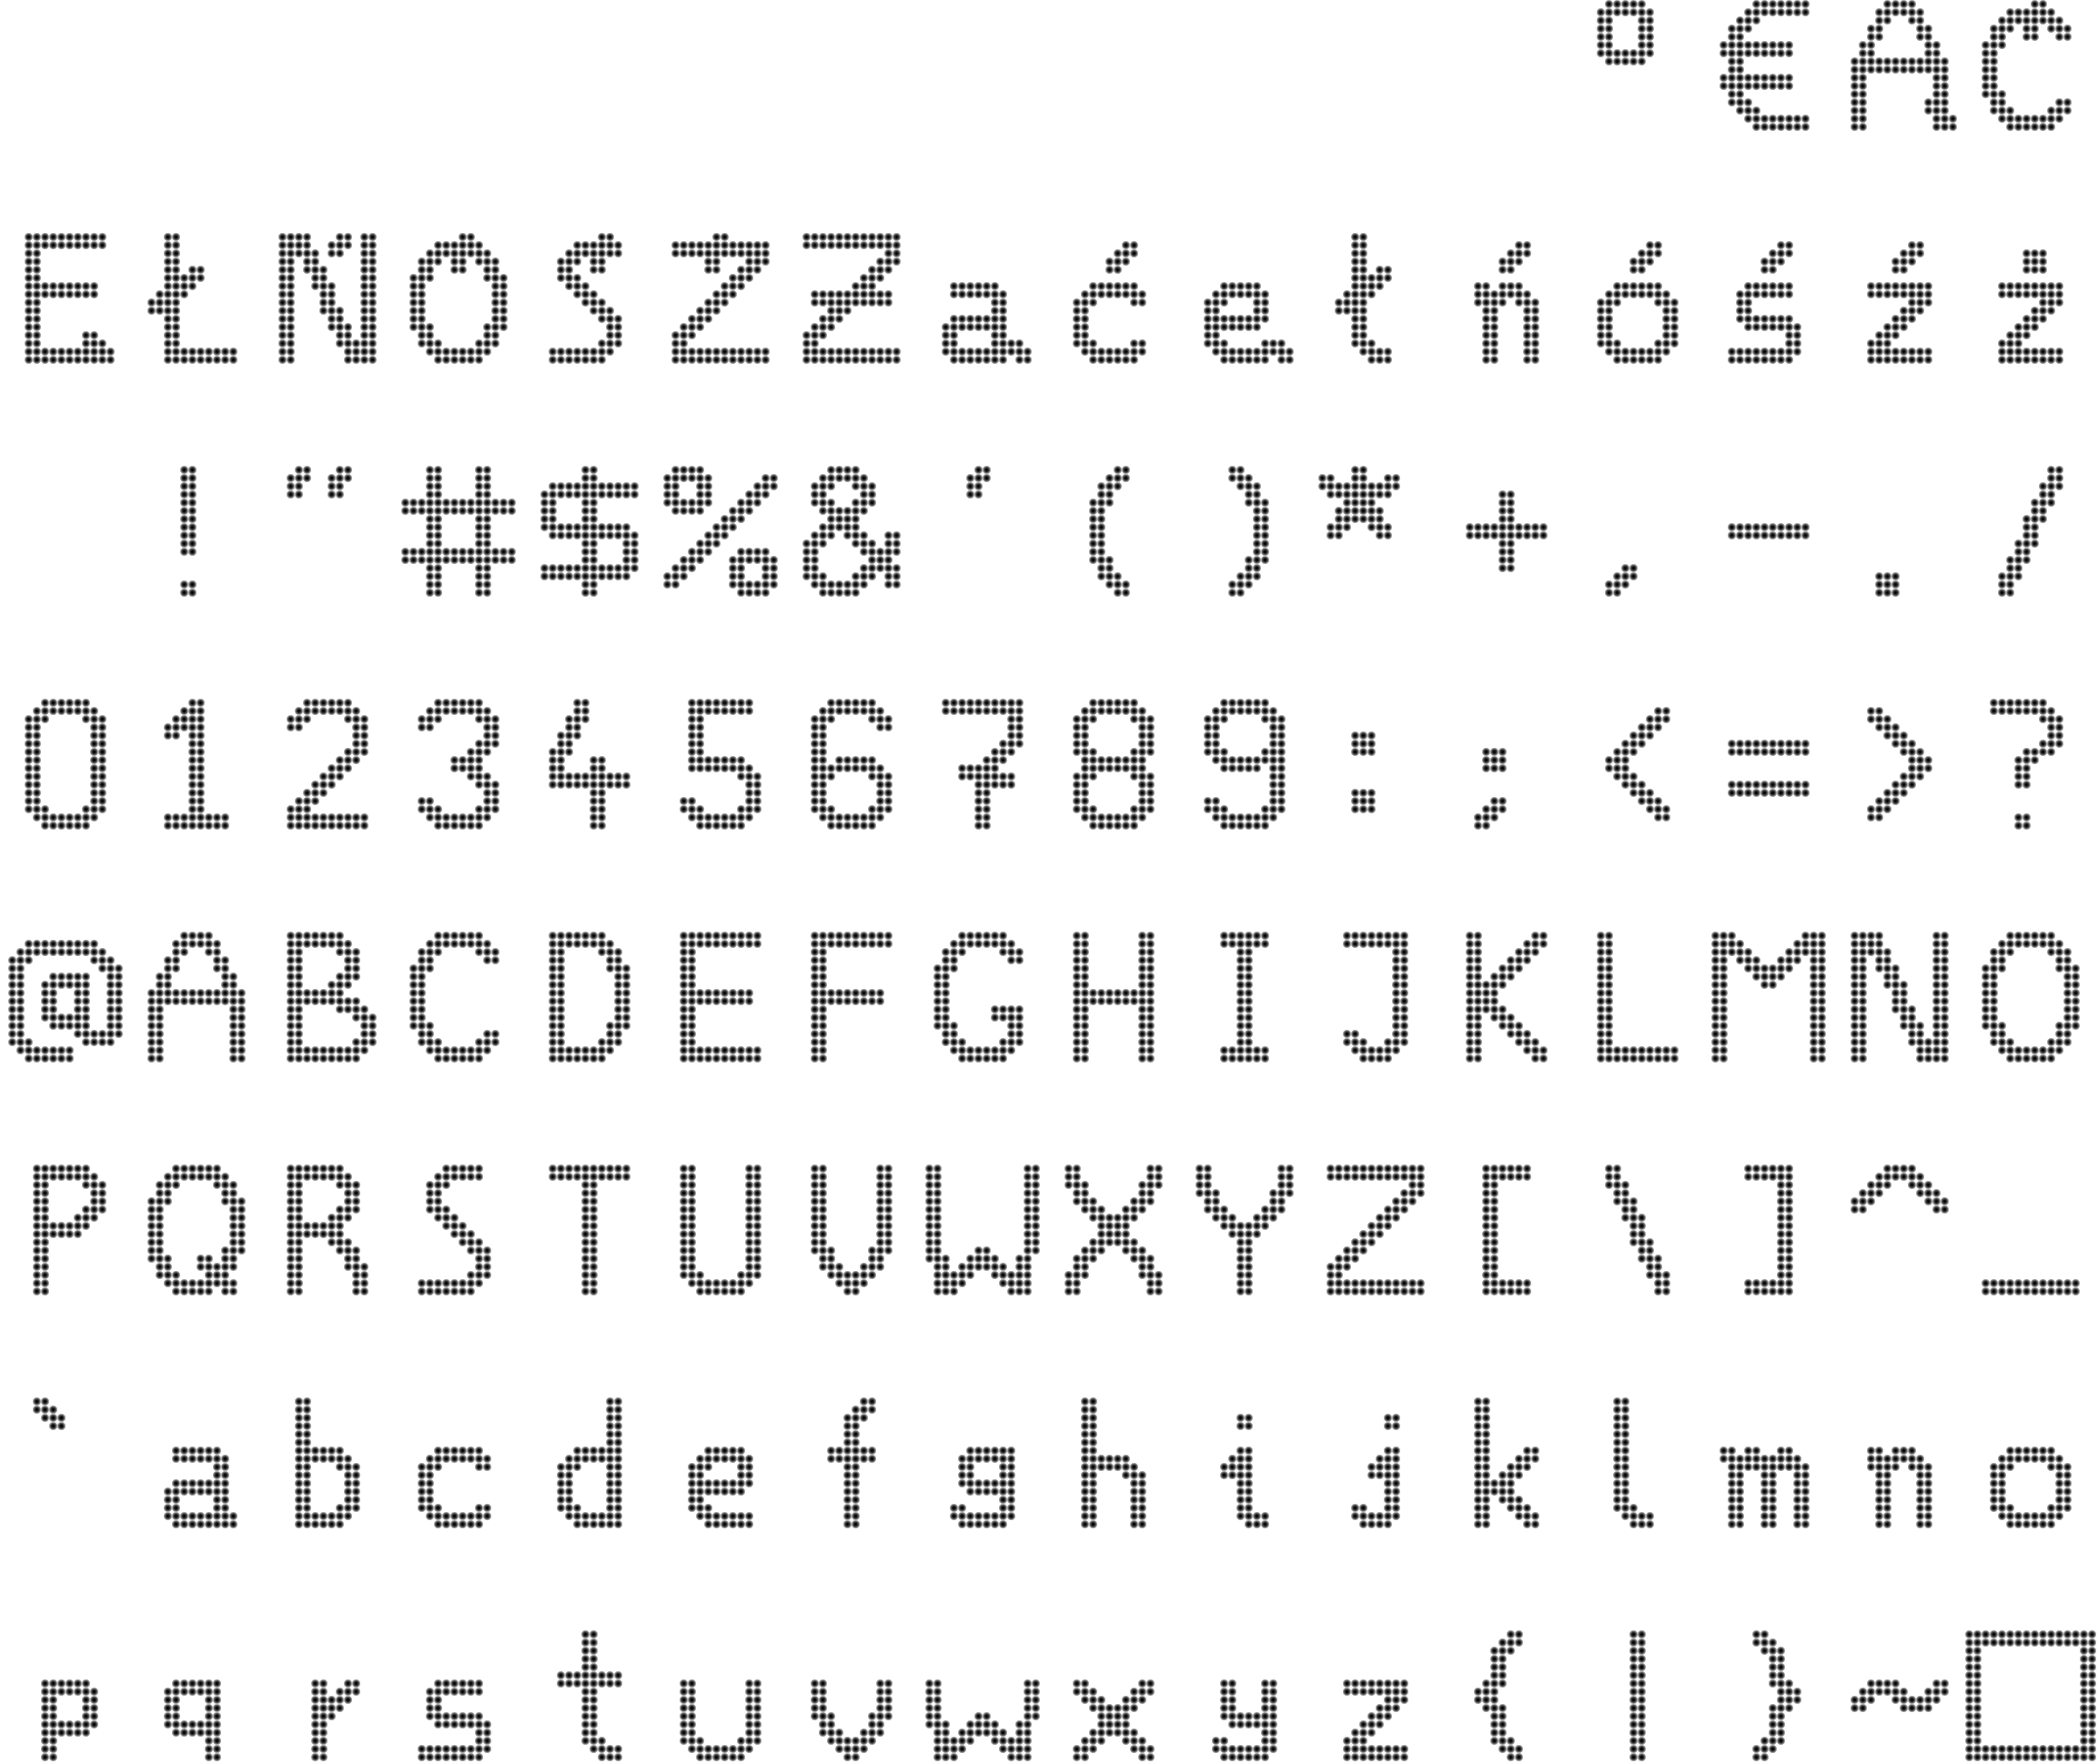
\includegraphics[width=250pt]{figures/czcionka0-praca.png}
	\end{center}
	\caption{Czcionka 0.}
\end{figure}

\textbf{Czcionka 1 ma rozmiar 8 px.} Celem utworzenia tej czcionki była możliwość wyświetlenia możliwie czytelnych dwóch linii tekstu. Wielkie litery i~cyfry mają jeden piksel odstępu od góry. Znaki z~elementami wystającymi w~górę korzystają z~tej przestrzeni. Ten odstęp również stanowi jednak przede wszystkim separację między liniami tekstu. Tak jak w~czcionce 0, linia dolna i~linia podstawowa są sobie równe.
\begin{figure}[htb]
	\begin{center}
		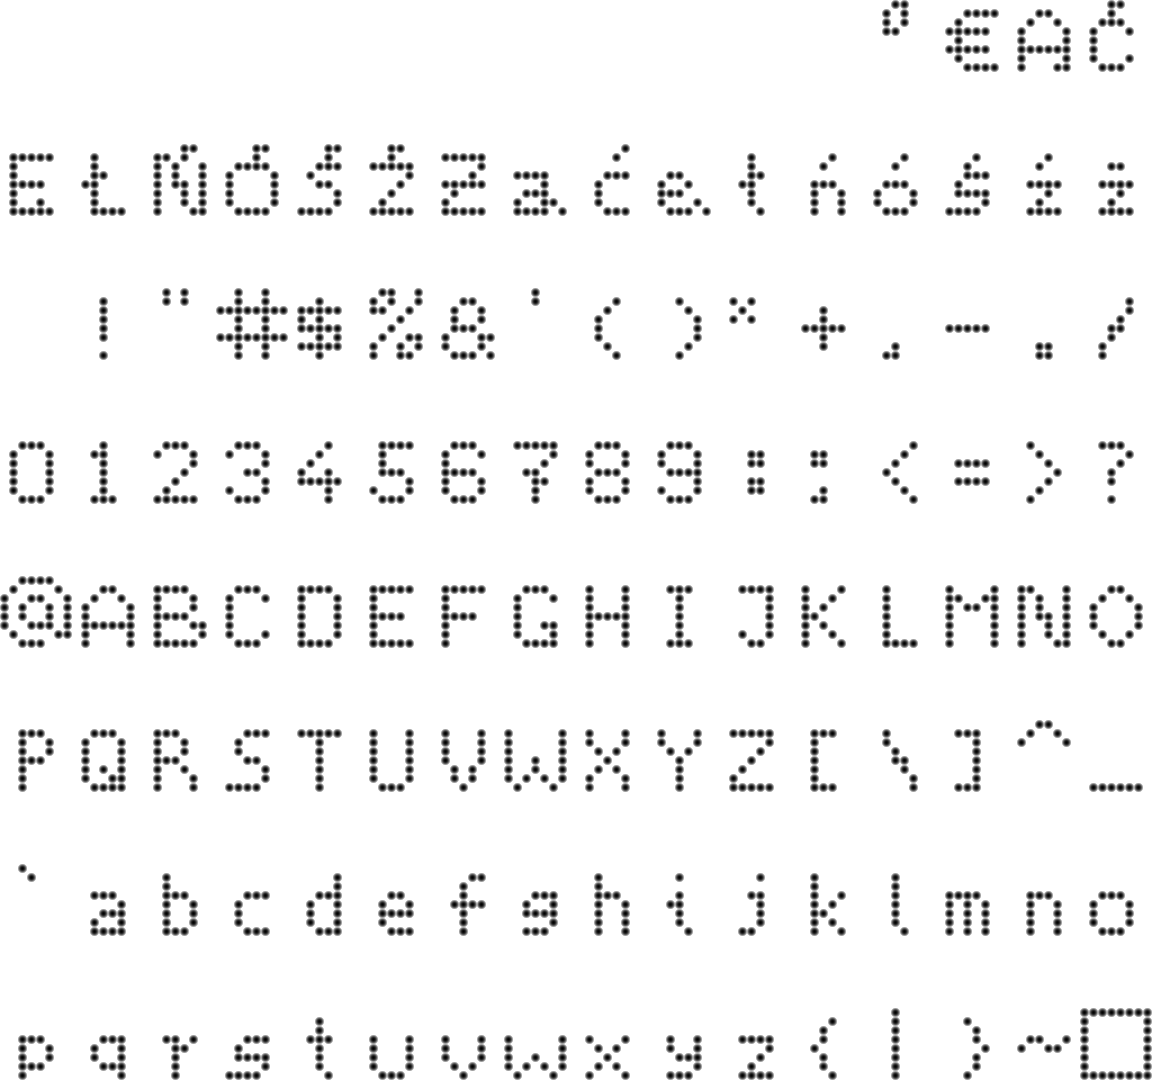
\includegraphics[width=200pt]{figures/czcionka1-praca.png}
	\end{center}
	\caption{Czcionka 1.}
\end{figure}

\textbf{Czcionka 2 ma rozmiar 12 px.} Bazuje na czcionce \textit{Fixedsys} zaprojektowanej przez Microsoft. Celem zastosowania tego fonta jest wypełnienie luki w~rozmiarach między tymi opisanymi wcześniej. Niektóre znaki w~tej czcionce były za wysokie i~zostały obniżone. Przez to również w~niej linia podstawowa nie we wszystkich znakach jest zachowana.
\begin{figure}[htb]
	\begin{center}
		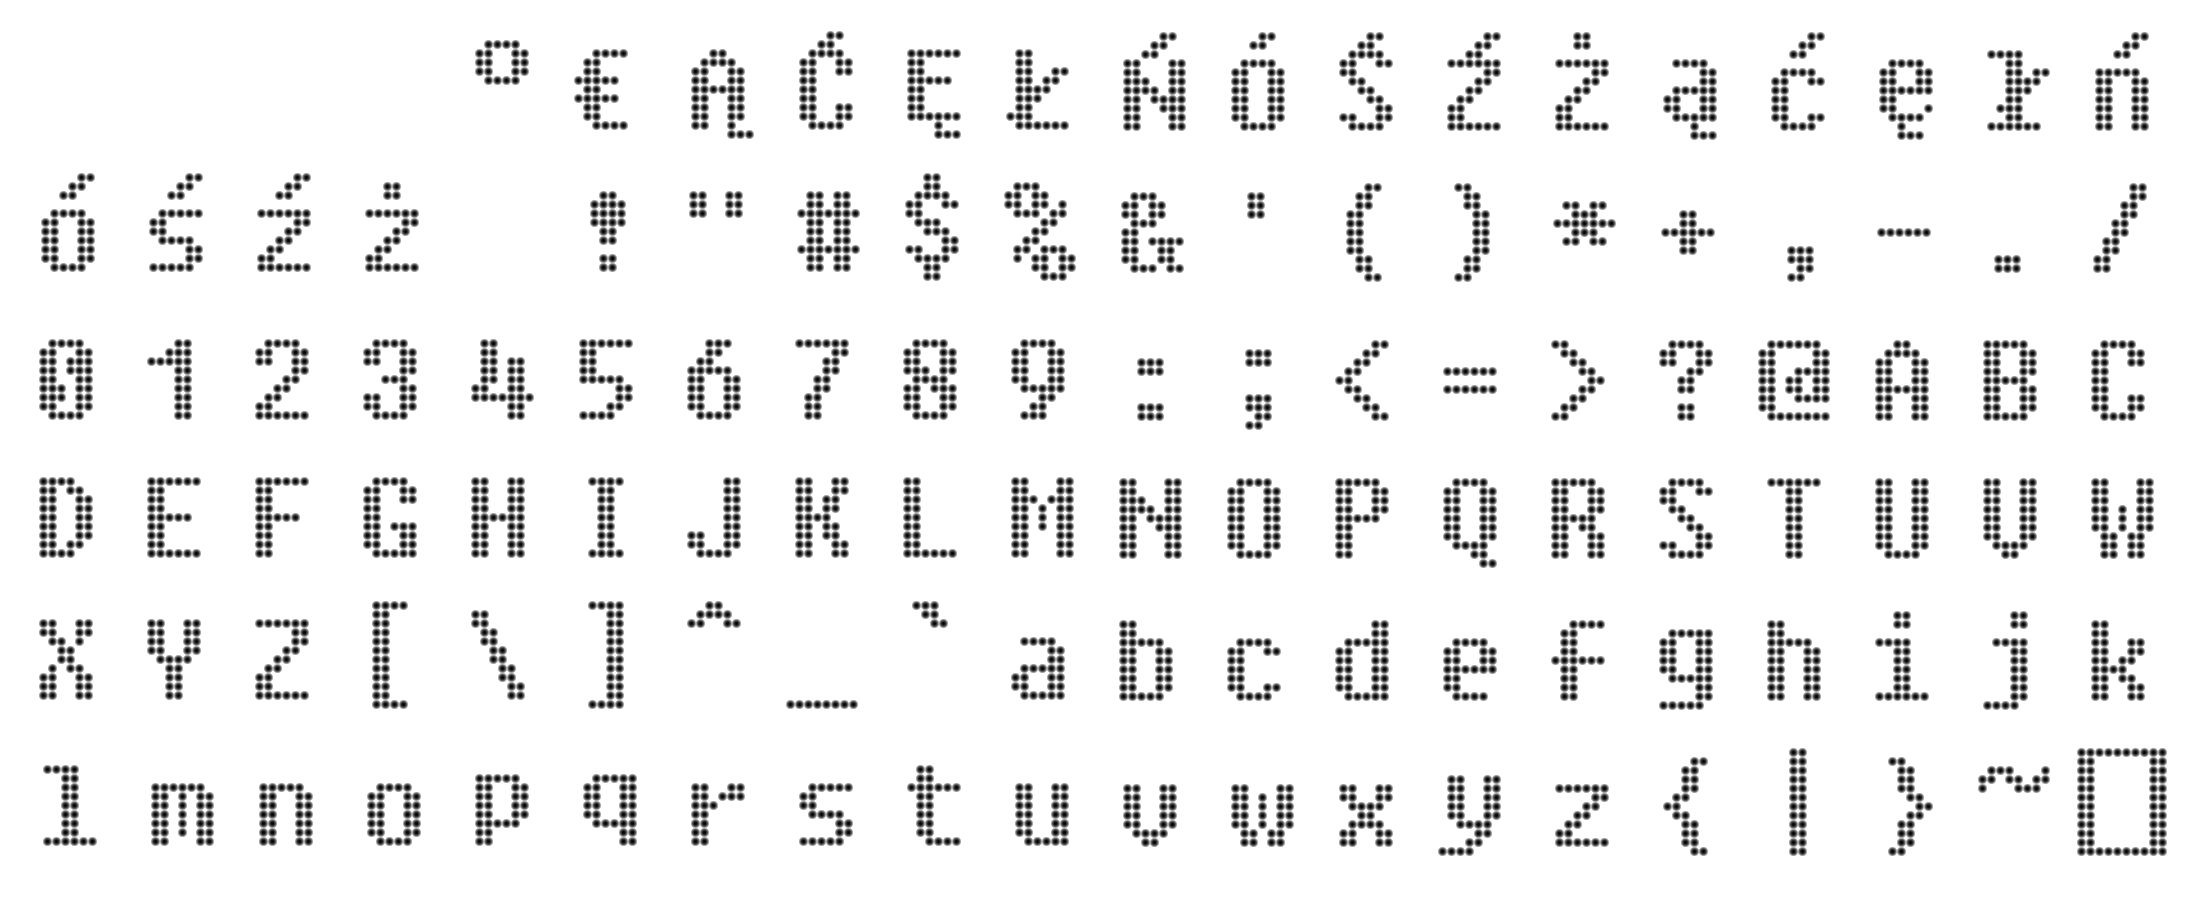
\includegraphics[width=300pt]{figures/czcionka2-praca.png}
	\end{center}
	\caption{Czcionka 2.}
\end{figure}

\newpage

\subsection{Szczegółowy opis działania}
\label{algorithm-description}
\subsubsection*{Stan początkowy}
\begin{enumerate}
	\item Tło jest wyczyszczone --- ustawiane na ciemne,
	\item rysowanie liter jest włączone,
	\item rysowanie tła jest wyłączone,
	\item gdy nie ma tła, zaczyna się od ciemnej klatki,
	\item ustawienie początkowe dla liter:
	\begin{enumerate}
		\item wszystkie litery są spacjami (kod 32),
		\item przycięcia są ustawione na OD = 0 i~DO = maksymalna wartość,
		\item tryb wyświetlania ustawiony na 0, czyli suma logiczna z~tłem, bez transpozycji o~przerzuceń,
		\item czcionka ustawiona na czcionkę 0, 16 pikseli.
	\end{enumerate}
\end{enumerate}

\subsubsection*{Algorytm}
\begin{enumerate}
	\item Czytaj komendy aż do natrafienia na komendę wymuszającą czekanie,
	\item zależnie od ustawień, kopiuj tło do bieżącej klatki, lub ustaw ją na pełną bądź pustą,
	\item po kolei, dla każdej litery o~numerze od 1 do 127 wykonuj zależnie od ustawień (kolejność ma znaczenie):
	\begin{enumerate}
		\item nadrzędną metodą ukrycia znaku jest ustawienie jego kodu na 32, czyli spację. Nawet w~trybie nadpisywania tła, taki znak zostanie pominięty,
		\item Transpozycja,
		\item Przerzucenie w~poziomie o~pionie,
		\item Przycięcia w~poziomie i~pionie,
		\item Rysowanie litery, modyfikując bieżącą klatkę.
	\end{enumerate}
	\item Przekaż bieżącą klatkę funkcji rysującej,
	\item czekaj do końca klatki, do końca 25~ms które powinna trwać,
	\item jeżeli nie nastąpiło oczekiwane zdarzenie (np. przycisk, zmiana godziny, narysowanie 100 klatek) przejdź do punktu 2,
	\item jeżeli nastąpiło oczekiwane zdarzenie przejdź do punktu 1.
\end{enumerate}

\subsection{Przykłady plików}
W poniższych przykładach przecinki i~spacje służą zwiększeniu czytelności zapisu, nie występują w~plikach. Liczby zostały zapisane w~systemie szesnastkowym.

Sekwencja 1:\\
{\small\texttt{02 01 10, 03 01 20, 04 01 30, 05 01 40, 06 01 50, 07 01 60, 08 01 70}}\\
oznacza rozmieszczenie znaków o~id od 1 do 8, w~odstępach co 16 pikseli.

Sekwencja 2:\\
{\small\texttt{01 00 65, 02 00 6B, 03 00 72, 04 00 61, 05 00 6E, 06 00 4C, 07 00 45, 08 00 44}}\\
przypisuje tym znakom kolejne litery ciągu ,,ekranLED''.
\begin{figure}[htb]
	\begin{center}
		
\includegraphics[width=300pt]{figures/screensample1.png}
	\end{center}
	\caption{Efekt odtworzenia przykładowej sekwencji 2.}
\end{figure}

Sekwencja 3:\\
{\small\texttt{01 03 0A, 02 03 04, 03 03 08, 04 04 01, 05 04 02, 06 05 04, 07 06 0D, 07 08 03,\\08 02 03}}\\
1. znak transponuje i~przerzuca w~pionie, 2. znak przerzuca w~poziomie, 3 znak przerzuca w~pionie, 4. znak zmienia na czcionkę 1, 5. znak zmienia na czcionkę 2, 6. znak rysuje od piątego piksela w~poziomie (4 odcięte), 7. znak jest rysowany od trzynastego piksela i~do trzeciego w~pionie, 8. znak jest przesunięty w~dół o~3 piksele.

\begin{figure}[htb]
	\begin{center}
		
\includegraphics[width=300pt]{figures/screensample2.png}
	\end{center}
	\caption{Efekt odtworzenia przykładowej sekwencji 3.}
\end{figure}

Sekwencja 4:\\
{\small\texttt{00 0E, 00 12 05 18 00 01 00 03 00 07 00 07 00 0F 00 0F 00 0F 00 1F 00 1F 00 1F 00 1F 00 3F 00 3F 00 3F 00 3F 00 3F 00 7F 00 7F 00 7F 00 7F 00 7F 00 7F 00 FF 00 FF 00 FF 00 FF 00 FF 00 FF 00 FF 01 FF 01 FF 01 FF 01 FF 01 FF 01 FF 01 FF 01 FF 03 FF 03 FF 03 FF 03 FF 03 FF 03 FF 03 FF 03 FF 03 FF 07 FF 07 FF}}\\
włącza rysowanie tła wyłączając rysowanie liter, oraz wczytuje tło przedstawione na rysunku.

\begin{figure}[htb]
	\begin{center}
		
\includegraphics[width=300pt]{figures/screensample3.png}
	\end{center}
	\caption{Efekt odtworzenia przykładowej sekwencji 4.}
\end{figure}

Sekwencja 5:\\
{\small\texttt{00 0F, 06 03 10, 07 03 01, 08 03 11, 00 14}}\\
włącza rysowanie znaków i~tła, 6. znak ustawia z~tryb nadpisywania tła, 7. znak w~tryb odjęcia od tła, 8 znak w~tryb alternatywy wykluczającej, oraz czeka na wciśnięcie przycisku.
\begin{figure}[htb]
	\begin{center}
		
\includegraphics[width=300pt]{figures/screensample4.png}
	\end{center}
	\caption{Efekt odtworzenia przykładowej sekwencji 5.}
\end{figure}

Prosty zegar:\\
{\small\texttt{02 01 10, 03 01 20, 04 01 30, 05 01 40, 01 00 00, 02 00 01, 03 00 3A, 04 00 02,\\05 00 03, 00 14}}\\
rozmieszcza znaki o~identyfikatorach od 1 do 7 co 16 pikseli, znakom 1 i~2 przypisuje dwucyfrową liczbę godzin, znakom 4 i~5 przypisuje dwucyfrową liczbę minut, znak 3 ustawia jako dwukropek, oraz czeka na wciśnięcie przycisku.

\begin{figure}[htb]
	\begin{center}
		
\includegraphics[width=300pt]{figures/screensample5.png}
	\end{center}
	\caption{Efekt odtworzenia przykładowej sekwencji 5.}
\end{figure}

\subsection{Pliki MXF}
\label{mxf-desc}
Pliki M2F maja skomplikowaną strukturę; podstawowy efekt, jakim jest przesuwający się w~poziomie tekst zostaje opisany dużym plikiem z~mnogością operacji. Wynika to z~konieczności zmieniania położenia każdego znaku w~każdej klatce, oraz przenoszenia wychodzących poza ekran znaków na początek. Przesunięcie o~jeden piksel tekstu, gdy jest widoczne 8 znaków, wymaga około 50 bajtów w~pliku M2F. W~związku z~tym został określony drugi format --- MXF.~Jego nazwa ma nawiązywać do formatu tekstowego TXT. W~przeciwieństwie do M2F, ten format charakteryzuje się daleko posuniętą prostotą.

Plik tego typu umożliwia wyłącznie wyświetlanie przesuwającego się w lewo tekstu. Kolejne znaki są czytane z~pliku i~umieszczane od prawej strony. Wykorzystana jest czcionka 0, o~wysokości 16 pikseli. Kodowanie znaków jest takie samo jak w~plikach M2F, co umożliwia wstawienie aktualnej godziny i~daty w~miejsce odpowiednich znaków sterujących.

Ze względu na sposób implementacji, w~którym narysowane znaki nie są modyfikowane, nie jest celowe wyświetlanie jedności sekund. Zamiast tego znaku (o~kodzie 5) jest wykonywana synchronizacja zegara z~zegarem czasu rzeczywistego. Gdyby zegar aktualizował się samoczynnie, wyświetlona godzina mogłaby być niespójna, zmienić się pomiędzy wstawieniem poszczególnych cyfr.

